% Based on the supplied article template, with a compact report layout.
\documentclass[a4paper]{article}
\usepackage[a4paper,margin=15mm]{geometry}
\usepackage[T1]{fontenc}
\usepackage[default]{sourcesans}
\pdfmapfile{=SourceSansThree.map}
\usepackage{microtype}
\usepackage{graphicx}
\usepackage{xcolor}
\usepackage{titlesec}
\definecolor{ink}{HTML}{182535}
\definecolor{muted}{HTML}{526171}
\definecolor{linkblue}{HTML}{0866C6}
\definecolor{rulegray}{HTML}{D8E0E8}
\usepackage[colorlinks=true,allcolors=linkblue]{hyperref}
\pagestyle{empty}
\setlength{\parindent}{0pt}
\setlength{\parskip}{2pt}
\setlength{\emergencystretch}{2em}
\titleformat{\section}{\color{ink}\bfseries\fontsize{11.5}{13.5}\selectfont}{}{0pt}{}
\titlespacing*{\section}{0pt}{7pt}{3pt}
\hypersetup{
  pdftitle={PhD Assignment Report},
  pdfauthor={Hashim Karim},
  pdfsubject={Temperature sensor selection, placement, integration and firmware improvements}
}

\begin{document}
\color{ink}
\fontsize{10.2}{12.2}\selectfont
\begin{minipage}[t]{0.60\linewidth}
\vspace{0pt}
{\fontsize{25}{28}\selectfont\bfseries PhD Assignment Report\par}
\end{minipage}\hfill
\begin{minipage}[t]{0.38\linewidth}
\vspace{0pt}
\raggedleft
{\fontsize{11}{13}\selectfont\bfseries Hashim Karim\par}
{\fontsize{9.3}{12}\selectfont
\href{mailto:h.karim-2@student.tudelft.nl}{h.karim-2@student.tudelft.nl}\\
\href{https://github.com/hashimkarim/densor}{github.com/hashimkarim/densor}\par}
\end{minipage}
\par\vspace{5pt}
{\color{linkblue}\hrule height 0.8pt}
\vspace{2pt}

\section*{Approach}
I extended Densor with external temperature sensing and independent sampling
rates. Revision 1 (R1) corrects baseline logging; Revision 2 (R2) and
Revision 3 (R3) introduce shared and partitioned multirate storage, respectively.

\section*{Sensor selection}
I considered an NTC thermistor, MAX30208, TMP117 and TMP119 for the 2.6--1.8~V
supply, prioritizing energy per reading. An NTC would require an accuracy budget
covering the thermistor, reference resistor and ADC, and possibly calibration.
\href{https://www.analog.com/media/en/technical-documentation/data-sheets/max30208.pdf\#page=8}{MAX30208}
offered lower conversion current, but its longer possible result latency could
extend the device's active time. I chose \textbf{TMP119} for factory-calibrated
I\textsuperscript{2}C readings, conversion energy similar to TMP117, tighter
specified accuracy and better tolerance to assembly and bending stress.
Professional assembly made its small package practical.

\par\vspace{5pt}
\begin{minipage}[t]{0.53\linewidth}
\vspace{0pt}
\section*{Sensor placement}
I placed TMP119 14.5~mm beyond the original board edge, with its 100~nF decoupling
capacitor nearby. The extension is intended to allow placement farther back in
the mouth, away from the main electronics. Literature examples favoured posterior
sites for reduced airflow effects
(\href{https://doi.org/10.1038/s41405-022-00114-8}{de Almeida e Bueno et al., 2022})
and greater temperature stability
(\href{https://doi.org/10.1016/j.rineng.2025.105284}{Zhao and Bergmann, 2025}).
\end{minipage}\hfill
\begin{minipage}[t]{0.44\linewidth}
\vspace{0pt}
\centering
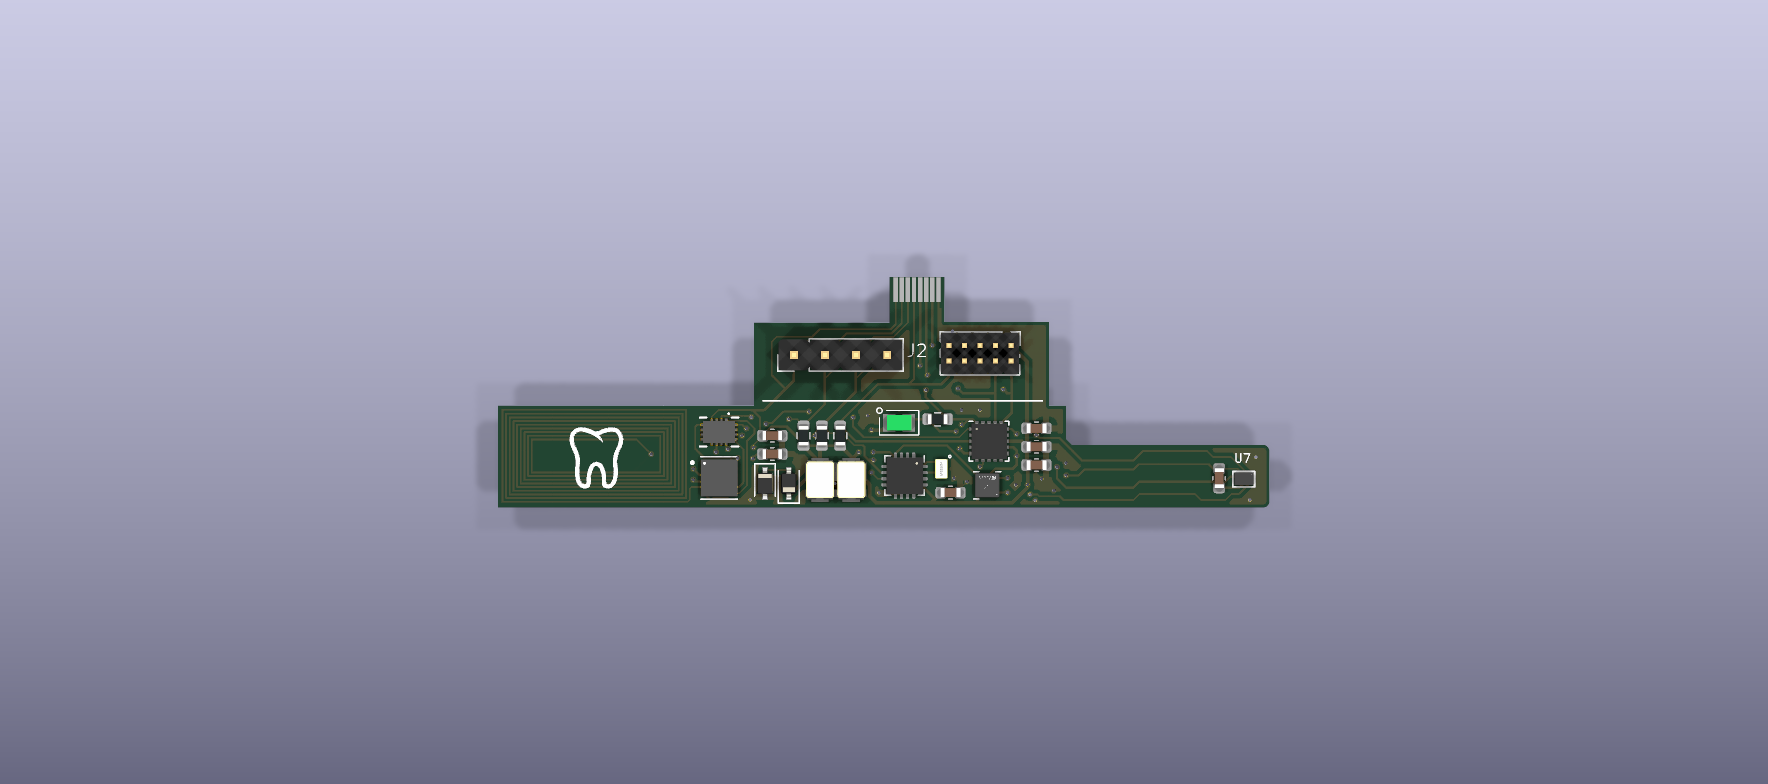
\includegraphics[width=\linewidth,trim=475bp 245bp 465bp 250bp,clip]{figures/pcb-top.png}
\par\vspace{3pt}
{\fontsize{8.5}{10}\selectfont\color{muted} Top-view PCB render. TMP119 (U7) sits at the right-hand tip of the extension.\par}
\end{minipage}

\section*{Firmware: temperature sensing and EEPROM logging}
At each RTC wake, firmware reads the sensors due, saves their data and powers
down. I added TMP119 \textbf{one-shot measurements without averaging} to shorten
active time: a conversion typically takes
\href{https://www.ti.com/lit/ds/symlink/tmp119.pdf\#page=14}{15.5~ms, versus 124~ms for eight averages}.
While TMP119 converts, firmware reads other due sensors, then collects its result
with a timeout. Users can select either temperature sensor or both; the log keeps
their readings separate, records supply voltage and reports missing sensors.

Extra EEPROM page writes cost energy. In R1, I moved the two-byte log pointer
from addresses 7--8 to 8--9 and aligned records to four-byte page boundaries.
This reduces avoidable page crossings at the cost of padding bytes. Firmware
checks that the record fits, waits for its writes to finish, then saves the new
pointer before powering off. If a write cannot be confirmed, it stops.

\section*{Firmware: multirate sampling}
Independent sampling rates allow frequent motion measurements without spending
energy on unnecessary temperature readings. The RTC wakes at the
\textbf{GCD} of the sensor periods; the finite-state machine (FSM) repeats after
their \textbf{LCM}. For temperature/photodiode/acceleration every 120/30/10~s,
the RTC wakes every 10~s: acceleration runs each tick, photodiode every 3 ticks
and temperature every 12 ticks. The cycle repeats after 12 ticks (120~s).
The FSM keeps its step in RTC RAM between MCU power cycles and advances after saving
the data.

\textbf{R2} stores samples together in shared memory; \textbf{R3} gives each
sensor its own region, sized in Android from record size and sampling rate and
fixed during a recording. Suffix \textbf{a} uses the retained FSM; \textbf{b}
calculates the sampling step from RTC time. Keeping the current write positions
in RTC RAM reduces EEPROM updates. Periodic EEPROM checkpoints save these positions
for recovery. Checksums help detect damaged records;
loss of timing stops the recording.

\section*{Android integration and visualization}
One Android app supports \textbf{R1, R2a, R2b, R3a and R3b}, with common-rate or
per-sensor settings. Settings take effect after firmware confirmation; checks
detect changes during NFC reads. Binary/CSV exports and temperature plots use
each sensor's sampling times.

I built \textbf{Sampling lab} to compare selected rates
against synthetic 100~Hz signals and export capacity-checked EEPROM images for
Android debug import. \textbf{EEPROM lab} compares records, padding, page crossings
and allocation across baseline/R1/R2/R3, with adjustable payloads and extra sensors
for packing experiments. These are simulations, not energy measurements.

Recorded checks include all four builds, firmware fault injection, 360 C-generated
images decoded in Java and 14 Android fixture tests on an S21 FE. Energy savings,
unaveraged temperature accuracy and physical power-loss behavior still require
board measurements.

\par\vspace{5pt}
{\color{rulegray}\hrule height 0.5pt}
\vspace{4pt}
{\fontsize{8.5}{10.5}\selectfont\color{muted}\textbf{AI usage.} I used AI for minor KiCad tasks (adding 3D
models and exporting files), literature review, repository documentation,
adapting the Android app to the
firmware using my open-source Android AI development tool,
\href{https://github.com/hashimkarim/android-agent-lab}{Android Agent Lab}, and
creating web apps to visualize EEPROM paging and sampling.\par}
\end{document}
